\usetikzlibrary{arrows,shapes,positioning,shadows,trees}

\tikzset{
  basic/.style  = {draw, rounded corners=2pt, thin, text width=10em, drop shadow, rectangle},
  root/.style   = {basic, align=center,
                   fill=blue!30},
  level 1/.style={level distance=5em},
  level 2/.style = {basic, align=center, fill=green!20, yshift=-2em},
  level 3/.style = {basic, rounded corners=2pt, thin, align=left, fill=pink!60, text width=16em, yshift=-2em}
}

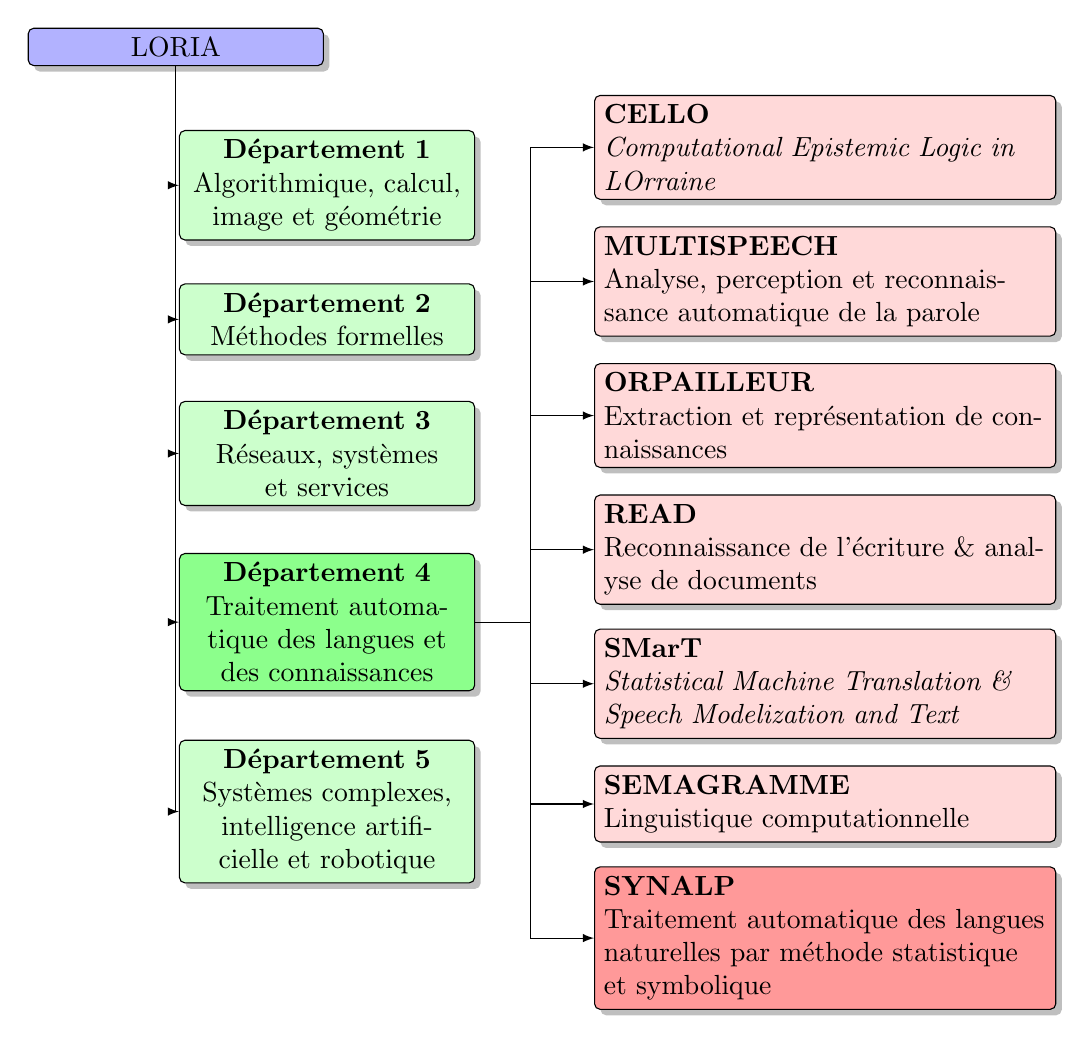
\begin{tikzpicture}[
  edge from parent path={[->](\tikzparentnode.south) -- ++(0,-0.5em)
			|- (\tikzchildnode.west)},
  >=latex]

% root of the the initial tree, level 1
\node[root](loria) {LORIA}
% The first level, as children of the initial tree
  child {node[level 2, , xshift=14em, yshift=2em] (c1) {\textbf{D\'{e}partement 1}\\Algorithmique, calcul, image et g\'{e}om\'{e}trie}}
  child {node[level 2, below of = c1] (c2) {\textbf{D\'{e}partement 2}\\M\'{e}thodes formelles}}
  child {node[level 2, below of = c2] (c3) {\textbf{D\'{e}partement 3}\\R\'{e}seaux, syst\`{e}mes et services}}
  child {node[level 2, below of = c3, fill=green!45!, yshift=-1.25em] (c4) {\textbf{D\'{e}partement 4}\\Traitement automatique des langues et des connaissances}}
  child {node[level 2, below of = c4, yshift=-2em] (c5) {\textbf{D\'{e}partement 5}\\Syst\`{e}mes complexes, intelligence artificielle et robotique}};

% The second level, relatively positioned nodes
\begin{scope}[every node/.style={level 3}]
% \node [below of = c1, xshift=1em] (c11) {Setting shape};
% \node [below of = c11] (c12) {Choosing color};
% \node [below of = c12] (c13) {Adding shading};
\node [below of = c4, xshift=18em, yshift=22em] (c41) {\textbf{CELLO}\\\textit{Computational Epistemic Logic in LOrraine}};
\node [below of = c41] (c42) {\textbf{MULTISPEECH}\\Analyse, perception et reconnaissance automatique de la parole};
\node [below of = c42] (c43) {\textbf{ORPAILLEUR}\\Extraction et représentation de connaissances};
\node [below of = c43] (c44) {\textbf{READ}\\Reconnaissance de l’écriture \& analyse de documents};
\node [below of = c44] (c45) {\textbf{SMarT}\\\textit{Statistical Machine Translation \& Speech Modelization and Text}};
\node [below of = c45, yshift=0.5em] (c46) {\textbf{SEMAGRAMME}\\Linguistique computationnelle};
\node [below of = c46, fill=red!40] (c47) {\textbf{SYNALP}\\Traitement automatique des langues naturelles par méthode statistique et symbolique};
\end{scope}

% lines from each level 1 node to every one of its "children"
% \foreach \value in {1,...,5}
%   \draw[->] (loria.south) -| (c\value.north);
\foreach \value in {1,...,7}
  \draw[->] (c4.east)  -- ++(2em,0em) |- (c4\value.west);
\end{tikzpicture}